In this section we would like to present an additional finding with respect to the
parsimonious nature \textit{PureCircuit} and \textbf{CLS} problems.
We define the following subclass of \textit{Tarski} \ref{def:tarski-ppad}:

\begin{definitionbox}{$\textit{KleeneTarski}$ problem definition}{kleene-tarski}
    Given $F: \mathbb{T}^n \to \mathbb{T}^n$, where $F$ is a \textit{natural} function \ref{def:nat-func},
    find $x \in \mathbb{T}^n$ such that $F(x) = x$.
    We assume $F$ will be represented as a circuit that uses set of gates
    $\{\wedge, \vee, \neg, \mathbf{0}, \mathbf{1}\}$.
\end{definitionbox}

Since the above problem abuses the fact that $F$ is \textit{natural} since that implies
that $F$ is monotone with respect to the partially ordered set $(\mathbb{T}^n, \preceq)$.
We show how this naturally results in a parsimonious reduction between \textit{PureCircuit}
and \textit{KleeneTarski}.

\begin{propositionbox}{Parsimonious Reduction between $\textit{KleeneTarski}$ and $\textit{PureCircuit}$}{kleene-pure}
    $$
        \textit{\#KleeneTarski} \subseteq \textit{\#PureCircuit}
    $$
\end{propositionbox}

\begin{proof}
    Given an input circuit $C: \mathbb{T}^n \to \mathbb{T}^n$, construct $\textit{PureCircuit}$ instance:
    \begin{enumerate}
        \item Initiate a vector of $n$ nodes, which we denote as $s$.
        \item Construct the $C$ using the standard set of gates and apply $C(x)$ to create output vector $o$.
        \item Copy the results back into $s$.
    \end{enumerate}

    \begin{figure}[h!]
        \centering
        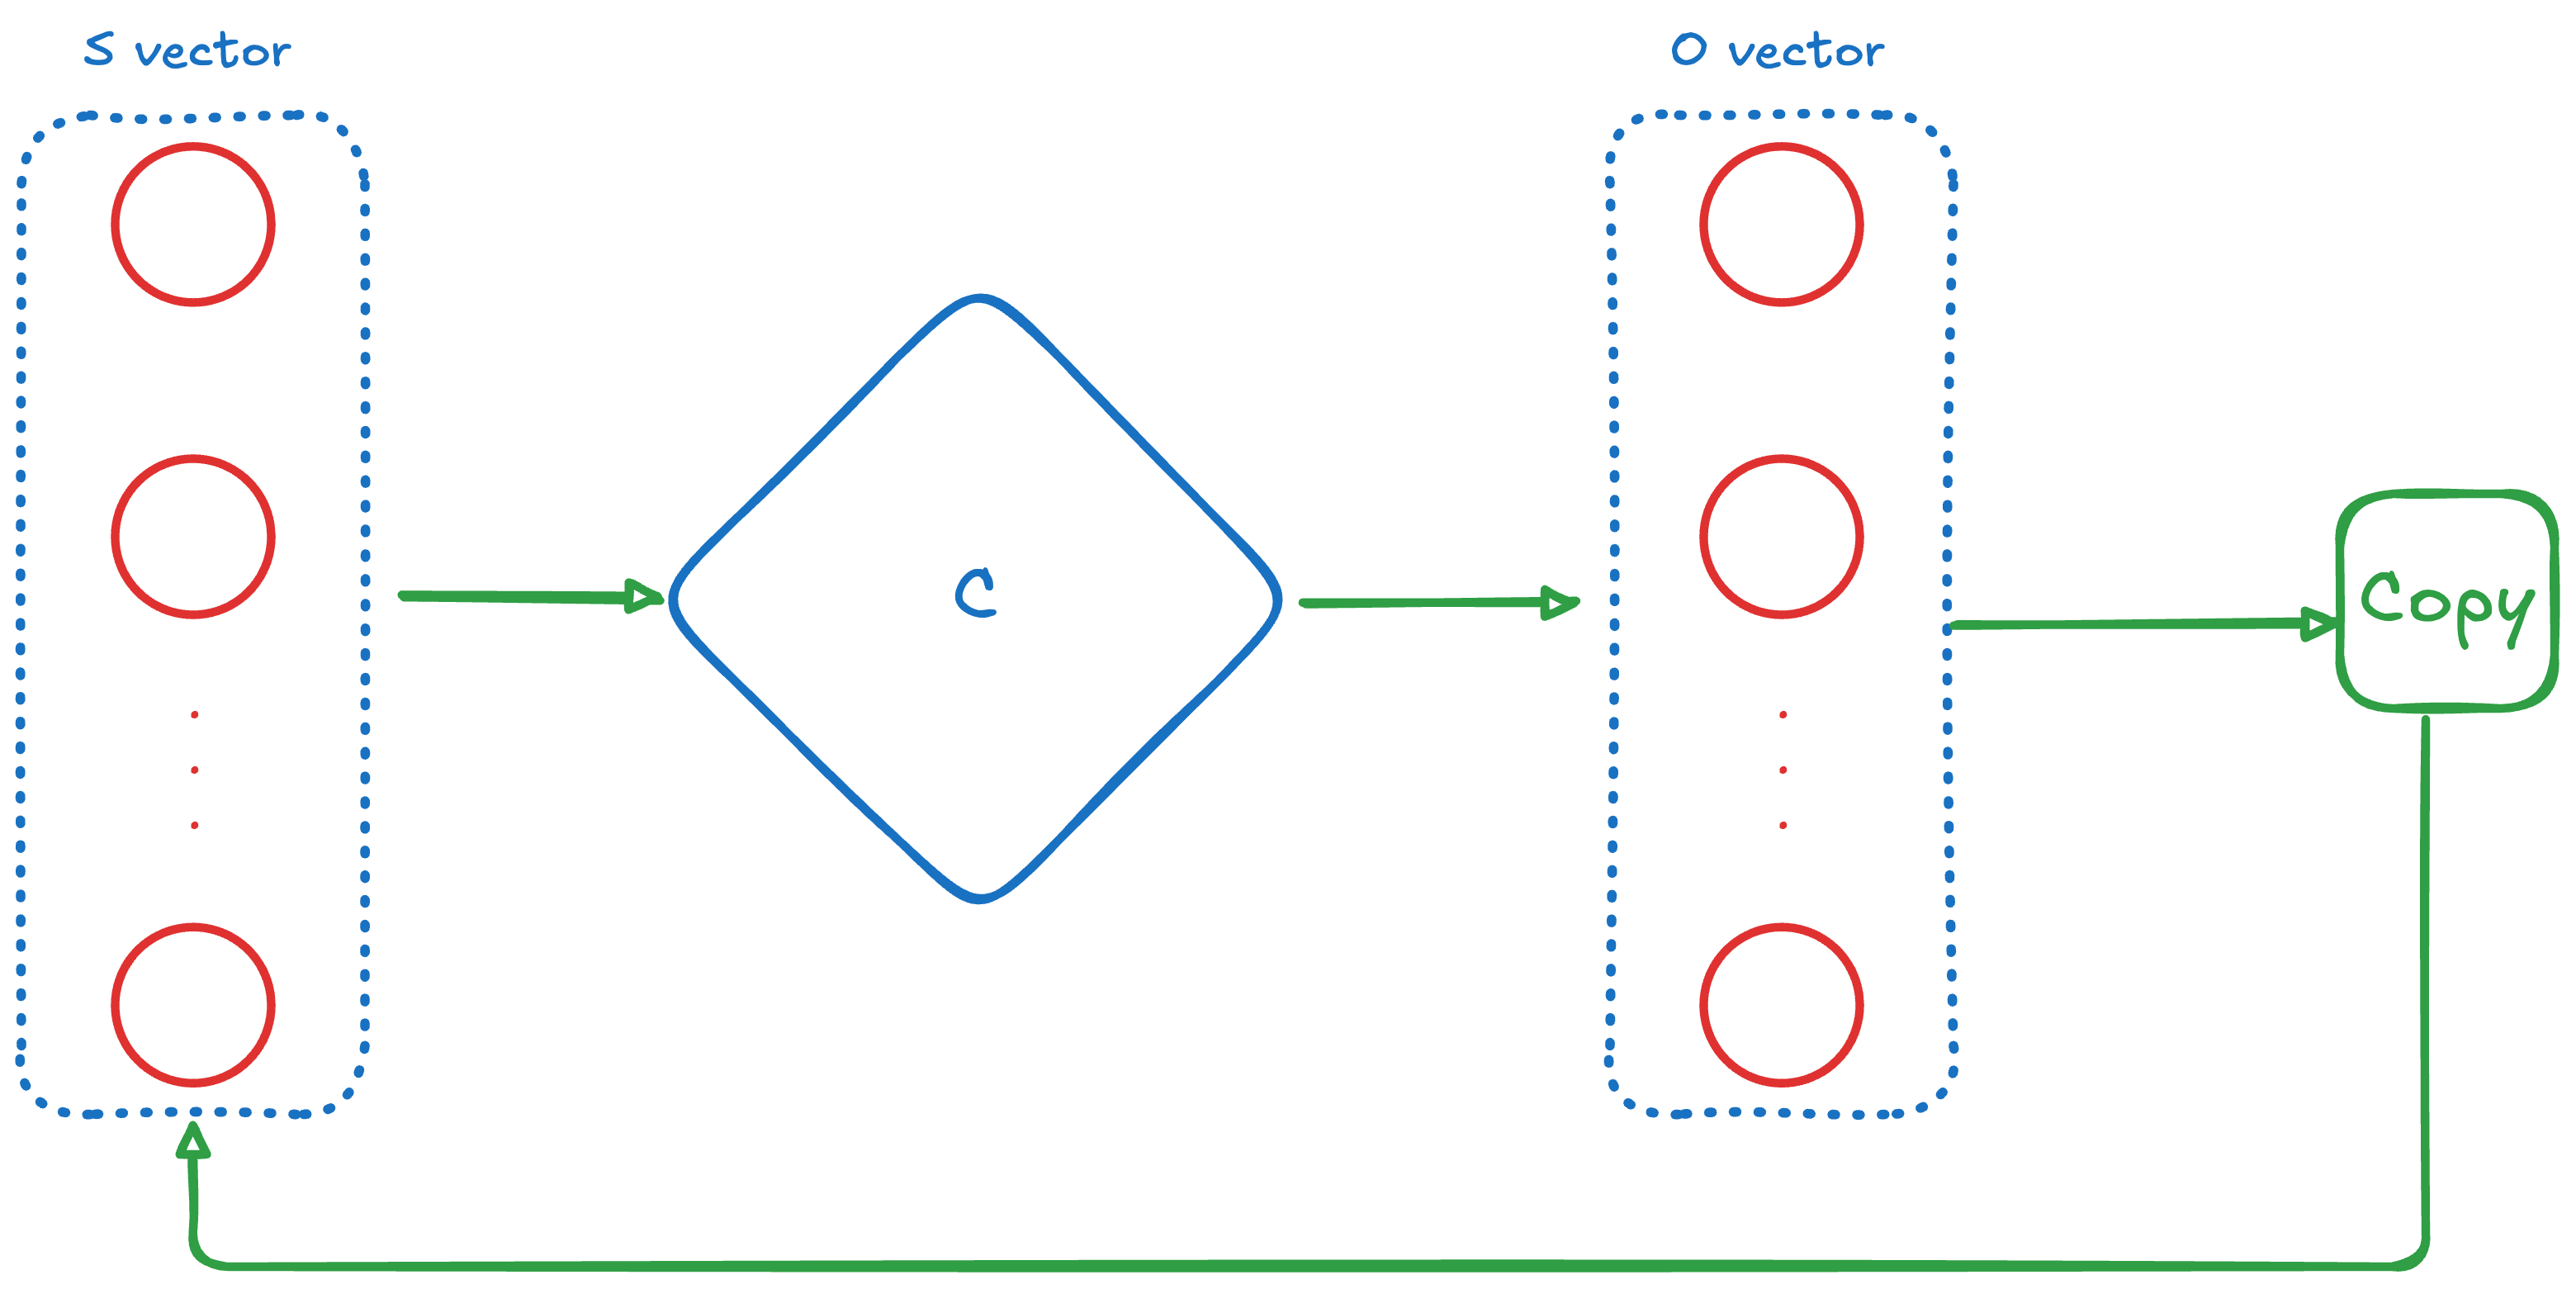
\includegraphics[width=0.5\textwidth]{assets/tarski-constrution.png}
        \caption[\textsc{KleeneTarski} construction]{\textsc{KleeneTarski} construction. Figure from interim report.}\label{fig:tarski-constr}
    \end{figure}


    We can visualise the above construction in figure \ref{fig:tarski-constr}.
    We can observe that, for any valid assignment $\mathbf{x} \implies \mathbf{x}[s]= \mathbf{x}[o]$,
    which implies $\mathbf{x}[o] = F(x) = \mathbf{x}[s]$.
\end{proof}

The above problem demonstrates how we can use \textit{PureCircuit}
to find fixed points in \textit{Tarski}. We expand
how we can built upon this idea to relate \textit{PureCircuit}
with ATMs
in our future works section \ref{sub-sub-sec:fw:pc-atms}\footnote{The above proposition and proof has been re-used from the interim report.}.



